
	Na het filteren van de hoeken kan het dus voorkomen dat er geen vier meer overblijven. Volgende kunnen hiervoor de oorzaak zijn. Enerzijds is het mogelijk dat bepaalde delen van schermen elkaar overlappen in de opstelling, anderzijds kunnen één of meerdere hoeken niet of slecht detecteerbaar zijn door een obstakel. Er wordt opgelegd dat minstens twee aanliggende hoekpunten en het middelpunt zichtbaar zijn. Indien men zich aan deze vooropgestelde eis houdt kan met volgend algoritme het scherm steeds volledig gereconstrueerd worden. Na een opsomming van de stappen volgt een meer gedetailleerde uitleg.
	\paragraph{Algoritme}
	 De input die wordt meegegeven is een dictionary van de reeds gevonden hoekpunten. De sleutels zijn LU,RU,RD en LD m.a.w. posities van hoeken en als bijhorende waarden coördinaten voor deze die reeds gevonden zijn en een \textit{null} als plaatshouder voor de nog te reconstrueren hoeken. \newline
	 Eerst worden de vier punten bepaald die zich rond het middelpunt op de diagonalen bevinden. Deze worden ook in een dictionary opgeslaan met dezelfde structuur als de input. Daarna wordt hoek per hoek gekeken welke nog ontbreken. Indien reconstructie nodig is, wordt het overeenkomende punt van de diagonalen genomen. Samen met het middelpunt wordt hieruit een eerste reconstructielijn opgesteld. Daarna wordt vanuit een aanliggend hoekpunt het laatste hulppunt bepaald waardoor de tweede rechte wordt getrokken. De gezochte hoek is dan het snijpunt van de twee constructielijnen. Deze stappen herhalen voor andere ontbrekende hoeken resulteert in een dictionary met alle hoekenpunten van het scherm. Hieronder volgt een uitgebreidere uitleg van gebruikte methodes met veronderstellingen, voordelen en nadelen.
	
	\subsection{Hulppunten op diagonalen} \label{subsec:diagonalen}
		
		Telkens wanneer reconstructie nodig is zulllen de punten op diagonalen rond het middelpunt bepaald en geordend opgeslaan worden in een dictionary. Hiervoor worden alle pixels overlopen die op de cirkel met een bepaalde radius rond het middelpunt liggen overlopen. De straal van deze cirkel wordt gedefiniëerd als een vierde van de grootste afstand tussen de reeds gevonden hoeken en het middelpunt. Op deze manier wordt rekening gehouden met de grootte van het scherm. 25 procent van deze afstand nemen zorgt ervoor dat de pixels niet tot het middelpunt behoren en er zich tegelijkertijd niet te ver van bevinden. 
		\paragraph{Startpunt} Het startpunt van waaruit de cirkel doorlopen wordt, is een pixel die niet tot een diagonaal behoord. Waarom dit belangrijk is zal later duidelijk worden. Bepalen of een punt deel uitmaakt van een diagonaal gebeurt aan de hand van een functie die controleerd of er zich tussen de desbetreffende pixel en een tweede meegegeven punt (in dit geval het middelpunt) een wit deel pixels bevindt. Indien er tussen de twee meegegeven punten een stuk wit voorkomt, betekend dit dat de pixel afkomstig is van een deel barcode \ref{Foto van screendetectie html!!!!} (*verwijzing foto van screendetectie html).
		Doordat de kleuren van de boord en diagonalen ook in de barcode voorkomen, sluit deze functie dus eigenlijk uit dat stukjes barcode toegevoegd worden aan de lijst. Het interval waarmee de hoek van nul tot twee keer pi loopt is één procent, hiermee worden net genoeg pixels overlopen. Naar later toe zou deze waarde ook relatief kunnen gezet worden naar de grootte van het scherm. Voor elke aaneenschakeling van pixels die geen wit kruisen op hun pad naar het middelpunt wordt een lijst aangemaakt tijdens het doorlopen van de cirkel. Uiteindelijk heeft men dan vier sublijsten van pixels in een lijst die elk een diagonaal voorstellen. Uit elke lijst wordt dan het middelste element genomen die het midden van dat cirkelsegment is. Hier komt al een eerste voordeel van het bepaalde startpunt naar voor. Indien dit niet gedaan zou worden kon het voorkomen dat een cirkel binnen een diagonaal startte. Dit zou resulteren in meer dan vier lijsten die aangemaakt worden wat het bepalen van de middens aanzienlijk complexer zou maken. 
		\paragraph{Ordenen} Zoals eerder vermeld worden deze vier punten dan vanuit een lijst geordend in een dictionary geplaatst. Als referentie wordt gestart vanuit de HTML voor de schermdetectie. Daarin zijn de twee bovenste hoeken geel en de onderste roze. Door de manier waarop de punten bepaald werden (het doorlopen van een cirkel) zitten de gele en roze pixels alreeds bij elkaar. Dus moet enkel nog gecontroleerd worden of de twee gele punten de eerste twee elementen in de rij zijn. Is dit niet het geval wordt de lijst geroteerd totdat aan de voorwaarde is voldaan. Elk element wordt dan in die volgorde toegevoegd aan de dictionary waardoor de punten telkens dezelfde ordening zullen hebben.
	
	\subsection{Reconstrueren van een hoekpunt}
		
		Indien een hoekpunt moet gereconstrueerd worden met andere woorden de waarde van de desbetreffende sleutel in de dictionary van hoekpunten is \textit{null}, zijn vier punten nodig waaruit twee rechten kunnen worden opgesteld waarvan het snijpunt dan de nieuwe hoek is. 
		\paragraph{Eerste hulppunt} In de daarnet aangemaakte dictionary wordt het punt op de diagonaal geselecteerd die hoort bij het ontbrekende hoekpunt. Als bijvoorbeeld de bijhorende waarde van LU \textit{null} is, wordt in de dictionary van punten op de diagonalen ook de waarde van LU geselecteerd.
		 Vanuit dit punt en het middelpunt kan de vergelijking voor een rechte opgesteld worden die de eerste constructielijn zal vormen. 
		 Een aanliggend hoekpunt met gekende coördinaat, hulphoek genaamd, zal door de voorwaarde van minstens twee aanliggende detecteerbare hoeken steeds gevonden worden. 
		Vanuit deze worden weer de cirkelsegmenten van boorden en diagonaal bepaald, dit met de radius die berekend werd in \ref{subsec:diagonalen}. Met als grote verschil dat nu niet de middens moeten bepaald worden maar de twee uiterste punten. Dit zullen dan de pixels zijn die op de rand van het scherm liggen. Hiervoor wordt van elk cirkelsegment het eerste en laatste element opgeslaan. Dit is meteen ook het tweede pluspunt van het startpunt, het zorgt ervoor dat de eerste en laatste pixel van de lijsten altijd de buitenste punten van een boord of diagonaal zijn. Dit stelt het mogelijk de lijst waarover geïtereerd moet worden te reduceren tot 6 pixels (2 punten per segment, 2 boorden en 1 diagonaal). De twee pixels die het verst van elkaar gelegen zijn zoeken in deze lijst is veel efficïenter dan alle punten van de segmenten te moeten overlopen. Door de offset en andere opgestapelde afrondingen kan het mogelijk zijn dat  kan het zijn dat op de rechte vanuit elke van deze punten naar de hulphoek pixels gekruist worden die niet dezelfde id hebben als dat punt van waaruit de rechte werd opgesteld. Indien dat het geval is wordt de dichtsbijzijnde pixel genomen op dat cirkelsegment waarvoor dit wel mogelijk is. \paragraph{Tweede hulpunt} Afhankelijk van de onderlinge ligging tussen het te reconstrueren hoekpunt en de hulphoek moet beslist worden welke van de twee berekende punten verder nodig zal zijn voor de reconstructie. Dit kan als volgt achterhaald worden. Ter referentie wordt eerst de rechte tussen hulp- en overstaande hoek van de te reconstrueren hoek bepaald. Dan wordt voor de twee te reduceren punten de rechte opgesteld met de hulphoek. Degene die de grootste hoek vormt samen met de referentie rechte, bevat het te behouden punt en deze vormt dan ook de tweede constructielijn. De nieuwe hoek wordt dan bekomen door het snijpunt van de twee constructielijnen te bepalen \cite{intersectie}. Om de id van de nieuw bepaalde hoek te bepalen, kan gekeken worden naar de tegenovergestelde hoek die reeds gekend zal zijn. Is die roze dan is de nieuwe hoek geel en vice versa. 
		
		\begin{figure}[H]
			\center
			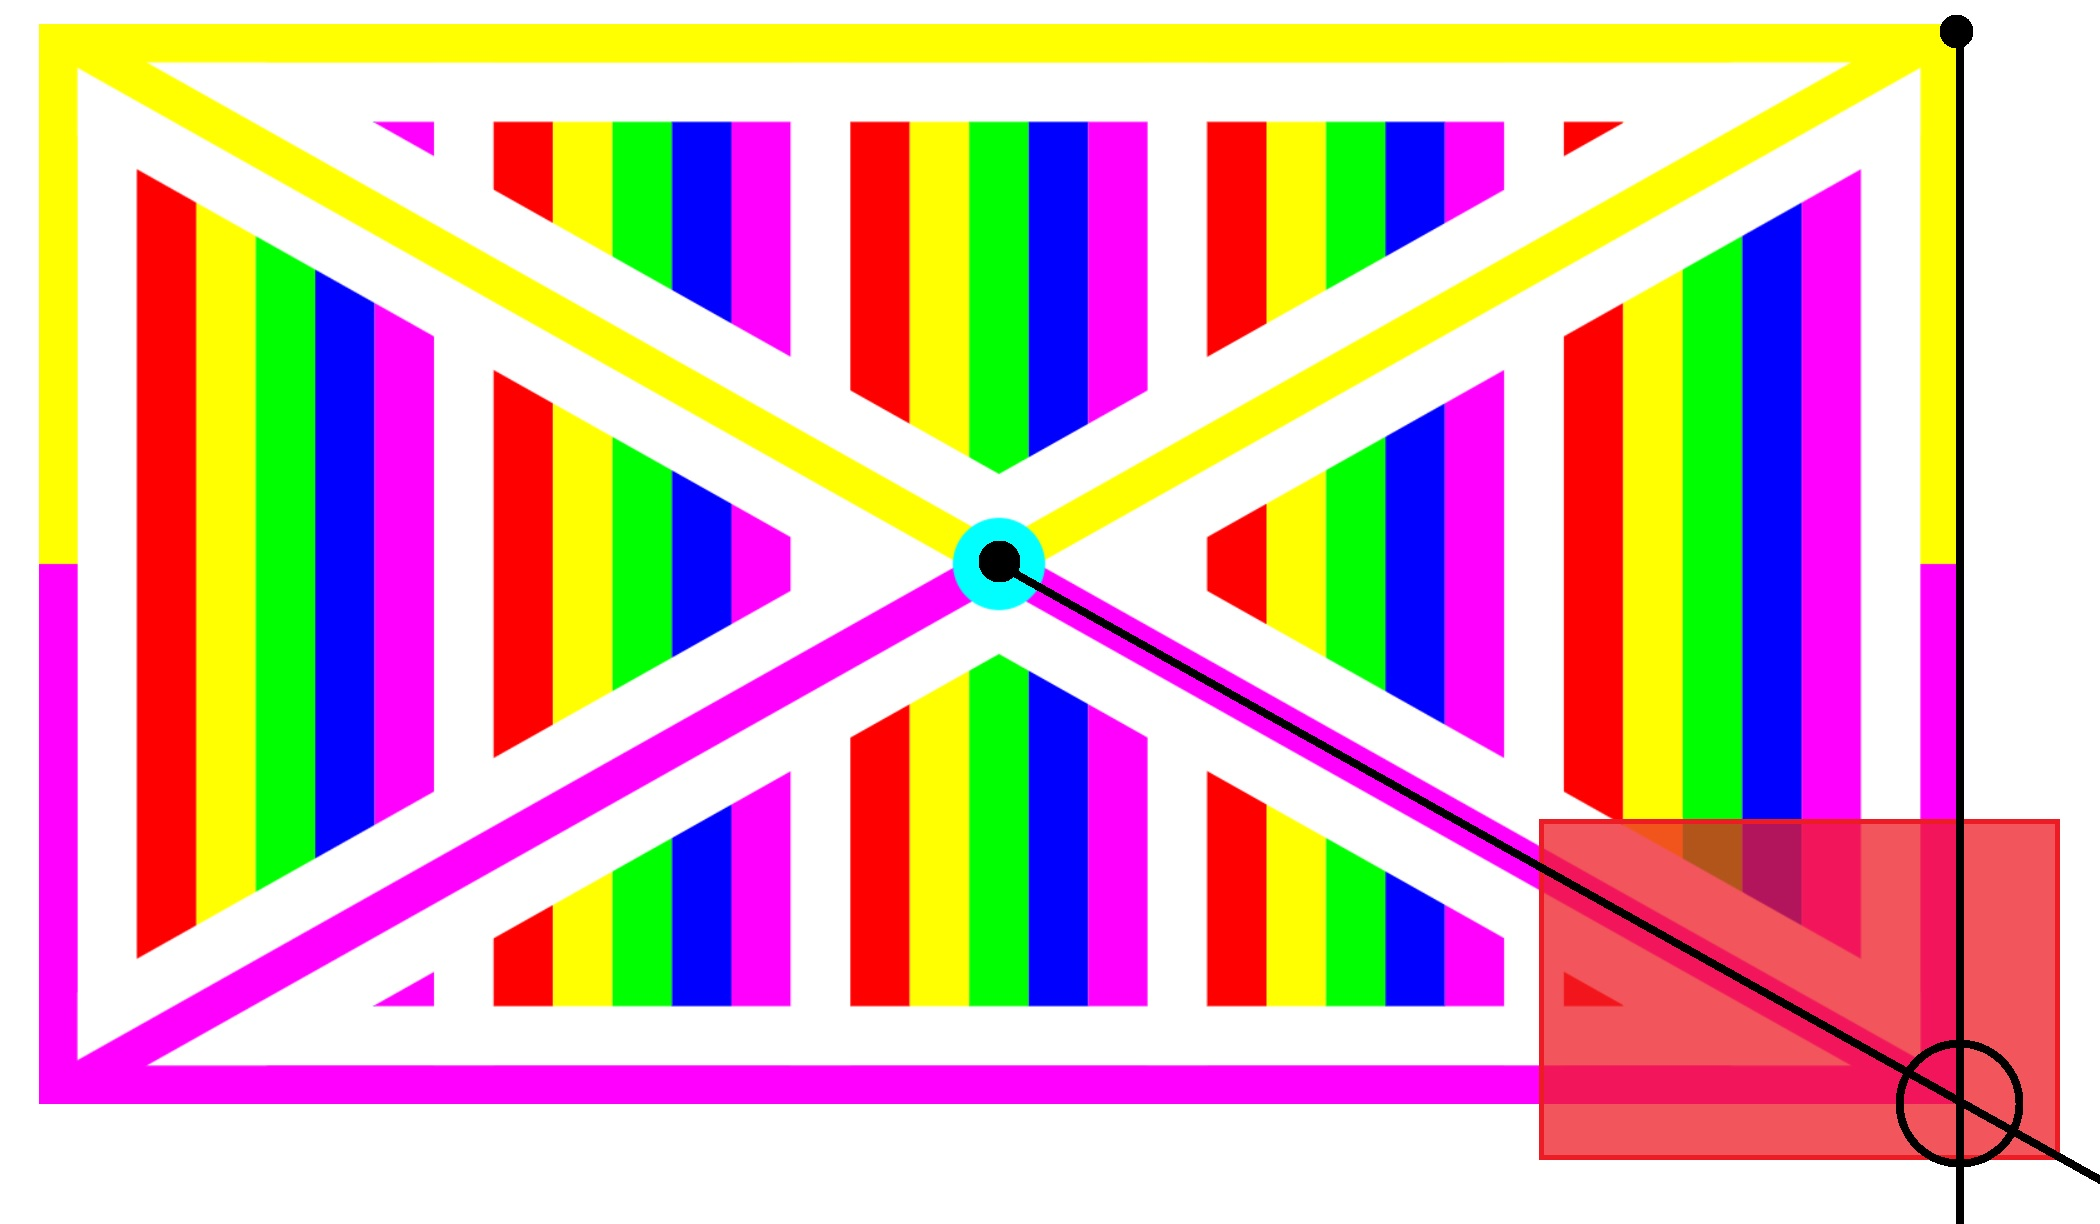
\includegraphics[width=0.8\textwidth]{img/screenReconstruction.jpg}
			\caption{Reconstructie van een hoekpunt. Zwarte punten zijn gebruikt, rode zijn ook berekend maar waren in deze situatie niet bruikbaar. Het rode vlak stelt de afdekking van de hoek voor.}
			\label{html}
			\label{scherm}
		\end{figure}
		
	